\documentclass[t]{beamer}

% Load general definitions
% Preamble file - general definitions, package loading, etc.

%=================================
% Load packages
\usepackage{amssymb,amsmath}
\usepackage{graphicx}
\usepackage{url}
\usepackage{tikz}
\usetikzlibrary{mindmap,trees,arrows}
\usepackage{fancyvrb}
\usepackage[english]{babel}
\usepackage[latin1]{inputenc}
\usepackage{subfigure}
\usepackage{times}
\usepackage[T1]{fontenc}
\usepackage{cancel}
\usepackage{color}
\usepackage{listings}

%=================================
% Set mode
\mode<presentation>
{
	\usetheme{Madrid}
	\usecolortheme{whale}
	\useoutertheme{infolines}
	\setbeamercovered{invisible}
}

% Get rid of nav bar
\beamertemplatenavigationsymbolsempty

% Insert frame number at bottom of the page.
\usefoottemplate{\hfil\tiny{\color{black!90}\insertframenumber}} 

%=================================
% Define new commands

\newcommand\Real{{\mathbb{R}}}
%\newcommand{\vi}{\vspace{0.6\baselineskip}}
%\newcommand{\goodgap}{\hspace{\subfigtopskip}\hspace{\subfigbottomskip}}


% Equation environments
\newcommand{\beq}{\begin{equation}}
\newcommand{\eq}{\end{equation}}
\newcommand{\beqs}{\begin{equation*}}
\newcommand{\eqs}{\end{equation*}}
\newcommand{\beqn}{\begin{eqnarray}}
\newcommand{\eqn}{\end{eqnarray}}

% Bold variables
\newcommand{\mbf}[1]{\ensuremath{\mathbf{#1}}}

% Itemization
\newcommand{\bitem}{\begin{itemize}}
\newcommand{\eitem}{\end{itemize}}
\newcommand{\spitem}{\vskip 1em\item}
\newcommand{\bitems}{\begin{itemize}\item}
\newcommand{\benums}{\begin{enumerate}\item}
\newcommand{\eenum}{\end{enumerate}}

% color blocks
\newenvironment{colorblock}[2]{%
\setbeamercolor{block title}{#2}
\begin{block}{#1}}{\end{block}}

% Vertical spacing
\newcommand{\vone}{\vskip 1em}
\newcommand{\vhalf}{\vskip .5em}

% Frame environments
\newenvironment{ftst}[3][t]{%
\begin{frame}{environment=ftst,#1}
\frametitle{#2}
\framesubtitle{#3}}{\end{frame}}

\newenvironment{ftstf}[2]{
\begin{frame}[fragile,environment=ftstf]
\frametitle{#1}
\framesubtitle{#2}}{\end{frame}}

% colors
\definecolor{MyGray}{rgb}{0.5,0.5,0.5}
\definecolor{MyDBGray}{rgb}{0.1,0.1,0.4}
\definecolor{darkgreen}{rgb}{0,0.4,0}
\definecolor{black}{rgb}{0,0,0}
\def\defn#1{{\color{red} #1}}

% Footnote
\renewcommand{\thefootnote}{\alph{footnote}}

% Relaxed footnotes
\newcommand{\lfr}[1]{\let\thefootnote\relax\footnote{\tiny #1}}

% Verbatim environment - using FANCYVRB package
\DefineVerbatimEnvironment%
{rcode}{Verbatim}
{fontsize=\scriptsize}

% Verbatim environment - using LISTINGS package
%\lstnewenvironment{rcode} {\lstset{	language = R,
%									basicstyle = \scriptsize\ttfamily,
%									showspaces = false,
%									showstringspaces = false,
%									showtabs = false,
%									keywordstyle = \color{black}\bfseries,
%									commentstyle = \color{darkgreen},
%									numbers = none,
%									otherkeywords={	<-,
%													ggplot,
%													geom_boxplot,
%													facet_grid,
%													shapiro.test,
%													fligner.test,
%													glht,
%													with},
%									deletekeywords={data,
%													model,
%													residuals,
%													c,
%													axis,
%													default,
%													labels,
%													qq.text}}}%
%{}


% Specific definitions
\title[]{Design and Analysis of Experiments}
\subtitle[]{05 - Statistical Inference}
\author[]{Felipe Campelo\\{\footnotesize http://orcslab.cpdee.ufmg.br/}}
\institute{Graduate Program in Electrical Engineering}
\date{\scriptsize Belo Horizonte\\April 2018}

\begin{document}

% cover page
\setbeamertemplate{footline}{}
\begin{frame}
\begin{flushright}

\includegraphics[width=.25\textwidth]{../figs/principal_completa3_ufmg}
\end{flushright}
  \titlepage
  \begin{tikzpicture}[remember picture,overlay]
  \node[anchor=south east,xshift=-5pt,yshift=122pt] at (current page.south east) {\tiny Version 2.12.2018};
  \node[anchor=south west,yshift=0pt] at (current page.south west) {
\includegraphics[width=.15\textwidth]{../figs/by-nc-sa.png}};
  \end{tikzpicture}  
\end{frame}

%=====

% quotation page
  \begin{frame}[b]
		\frametitle{}
\begin{columns}[T]
\column{0.65\textwidth}
\flushright{\small ``\textit{Nothing in life is to be feared,\\
it is only to be understood.\\
Now is the time to understand more,\\
so that we may fear less.}''
\vskip 5em
Marie Sklodowska Curie\\
1867--1934\\
Polish-French physicist and chemist.\\}
\column{0.35\textwidth}
\begin{tikzpicture}[remember picture,overlay]
\node[anchor=south east,yshift=15pt,xshift=0pt] at (current page.south east)
{
\includegraphics[width=\textwidth]{../figs/curie.jpg}};
\end{tikzpicture}
\end{columns}
\vhalf
\lfr{Image: \url{http://mariecurietpe.unblog.fr}}
\end{frame}

%=====

% Main slides
\begin{ftst}
{Statistical Inference}
{Introduction}
Definitions such as point estimators and statistical intervals belong to a branch of statistical theory known as \textit{descriptive statistics}, that is, methods that are focused on accurately describing characteristics such as location or uncertainty about a given population parameter;
\vone
While these concepts are certainly important, in many cases description is not enough -- one may need decision-making tools to deal with information from random samples, tools that allow a researcher to perform \textit{inference} with a quantifiable degree of certainty.
\end{ftst}

%=====

\begin{ftst}
{Statistical hypotheses}
{Scientific Hypotheses}
A \textit{hypothesis} is a proposed explanation for an observable phenomenon.
\vone
Scientific hypotheses must satisfy (at least) two conditions:

\bitems Falsifiability;
	\item Testability;
\eitem
\vone
\begin{columns}[T]
    \column{0.75\textwidth}
	\begin{colorblock}{}{bg=green!30,fg=black}
	``\textit{The more we learn about the world, and the deeper\\
	our learning, the more conscious, specific,\\
	and articulate will be our knowledge of what\\
	we do not know, our knowledge of our ignorance.}''\\
	\flushright\vspace{-1em}\small Sir Karl R. Popper\\
	\flushright\vspace{-1em}\small (1902-1994)\\
	\flushright\vspace{-1em}\small Austro-British philosopher
	\end{colorblock}
	\column{0.25\textwidth}
\begin{tikzpicture}[remember picture,overlay]
\node[anchor=south east,yshift=13pt,xshift=0pt] at (current page.south east) {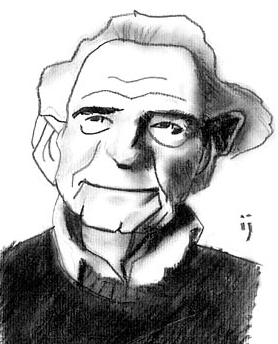
\includegraphics[width=\textwidth]{../figs/popper.png}};
%\node[anchor=south east,yshift=0pt,xshift=-15pt] at (current page.south east) {Karl Popper};
\end{tikzpicture}
\end{columns}
\lfr{Image: Copyright 2008 Ivan Jer\^onimo \url{http://www.ivanjeronimo.com.br}}
\end{ftst}

%=====

\begin{ftst}
{Statistical Hypothesis}
{The hypothetico-deductive model}
The \textit{hypothetico-deductive model} of construction of scientific knowledge includes:

\bitems Formulation of falsifiable hypotheses;
	\item Refutation or corroboration of the hypotheses by the data;
	\item Comparison between alternative hypotheses - principle of parsimony (Ockham's razor);
	\item Predictive power;
\eitem

\begin{columns}[T]
	\column{0.20\textwidth}
\begin{tikzpicture}[remember picture,overlay]
\node[anchor=south west,yshift=20pt,xshift=15pt] at (current page.south west) {
\includegraphics[width=.7\textwidth]{../figs/ockham2.png}};
\end{tikzpicture}
    \column{0.80\textwidth}
    \vhalf
	\begin{colorblock}{}{bg=green!30,fg=black}
	``\textit{Numquam ponenda est pluralitas sine necessitate.}''\\
	\flushright\vspace{-1em}\small William of Ockham\\
	\flushright\vspace{-1em}\small (1287-1347)\\
	\flushright\vspace{-1em}\small English philosopher and theologian\\
	\end{colorblock}
\end{columns}
\lfr{Image: \url{http://www.philosophybasics.com/philosophers_ockham.html}}
\end{ftst}


%=====

\begin{ftst}
{Statistical Hypotheses}
{Definitions}
\textit{Statistical hypotheses} are defined as objective statements about parameters of one ore more populations;
\vone
\textbf{Attention}: the statements in statistical hypotheses are about parameters of the \textit{population} or \textit{model}, \textbf{not the \textit{sample}}.
\vone
On frequentist approaches, the formal test of hypotheses involves the contrast between \textit{null} and \textit{alternative} hypotheses.
\begin{columns}[T]
	\column{0.48\textwidth}
	\begin{block}{Null hypothesis ($H_0$)}
	\small
	\bitems Absence of effects;
	\item \textit{Conservative} model.\eitem
	\textbf{Example:} $H_0: \mu = 25$
	\end{block}
	\column{0.48\textwidth}
	\begin{block}{Alternative hypothesis ($H_1$)}
	\small 
	\bitems Presence of some effect;
	\item Existence of something ``new''.\eitem
	\textbf{Example:} $H_1: \mu \neq 25$
		\end{block}
	\end{columns}
\end{ftst}

%=====

\begin{ftst}
{Statistical Hypotheses}
{Definitions}
Determination of the reference value for the null hypothesis $H_0$:

\bitems Previous knowledge about the process (investigation of changes);
	\item Value obtained from theory or models (model validation);
	\item Project requirements (investigation of system compliance);
\eitem
\vone
Hypothesis testing involves:

\bitems Obtaining the sample;
	\item Calculation of test statistics;
	\item Decision based on the computed value;
\eitem
\end{ftst}

%=====

\begin{ftst}
{Statistical Hypotheses}
{Example}
Suppose you own a company that sells green peas to large customers, 
and that you want to determine whether your $50$kg sacks really 
contain their nominal weight (at least on average).
\vhalf
In this case the null hypothesis could be defined as:
\textit{the average net weight of a sack is $50$kg}, and the alternative of interest could be expressed as the complementary inequality.
\beqs\begin{cases}
H_0: \mu = 50kg \\
H_1: \mu \neq 50kg 
\end{cases}\eqs
\vone
Suppose still that $n = 10$ packs are randomly sampled, and their contents are weighted using a calibrated scale;
\begin{tikzpicture}[remember picture,overlay]
\node[anchor=north east,yshift=12pt,xshift=-5pt] at (current page.north east) {
\includegraphics[width=0.2\textwidth]{../figs/peas.png}};
\end{tikzpicture}
\lfr{Image: \url{http://www.storko.eu/ed_files/image/green-peas.jpg}}
\end{ftst}

%=====

\begin{ftst}
{Statistical Hypotheses}
{Example}
Since the sample mean $\bar{x}$ is a good estimator of the real mean $\mu$, common sense suggests that:

\bitems If $\bar{x} \cong 50$kg - corroboration of $H_0$;
\item If $\bar{x} \ll 50$kg or $\bar{x} \gg 50$kg - refutation of $H_0$;
\eitem
\vone
That is, we can use $\bar{x}$ as the basis for a statistical test.
\vone
But how to define a \textit{critical region} for the rejection of $H_0$?
\vone\vhalf
\centering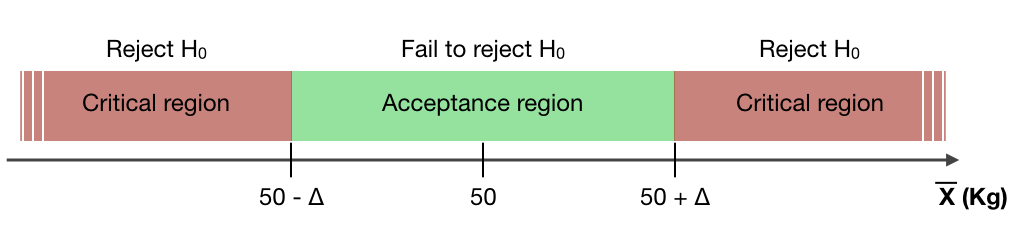
\includegraphics[width=\textwidth]{../figs/regcrit.png}
\begin{tikzpicture}[remember picture,overlay]
\node[anchor=north east,yshift=12pt,xshift=-5pt] at (current page.north east) {
\includegraphics[width=0.2\textwidth]{../figs/peas.png}};
\end{tikzpicture}
\end{ftst}

%=====

\begin{ftst}
{Inferential Errors}
{Type I error}
\begin{colorblock}{}{bg=green!30,fg=black}
\textbf{Type I error} (false positive): rejecting the null hypothesis when it is true.
\end{colorblock}
\vone
The probability of occurrence of a false positive in any hypothesis testing procedure is generally known as the \textit{significance level} of the test, represented by Greek letter $\alpha$:
\beqs \alpha = P\left(\mbox{type I error}\right) = P\left(\mbox{reject }H_0|H_0\mbox{ is true}\right)\eqs
\vone
Another frequently used term is the \textit{confidence level} of the test, given by $(1-\alpha)$.
\end{ftst}

%=====

\begin{ftst}
{Inferential Errors}
{Type I error}
For a given sample, the selected value of $\alpha$ defines the critical threshold for the rejection of $H_0$.
\vone
If $H_0$ is true (i.e., if $\mu=50$kg), the distribution of values of $\bar{x}$ is aproximately normal (assuming the CLT holds), with average $50$kg and standard error $(\sigma/\sqrt{n})$ kg;
\vone
For a desired Type-I error probability $\alpha=0.05$, the critical values of the distribution of $\bar{x}$ are the ones for which the probability content within the acceptance region under the null hypothesis is $1-\alpha = 0.95$.
\begin{tikzpicture}[remember picture,overlay]
\node[anchor=south east,yshift=0pt,xshift=0pt] at (current page.south east) {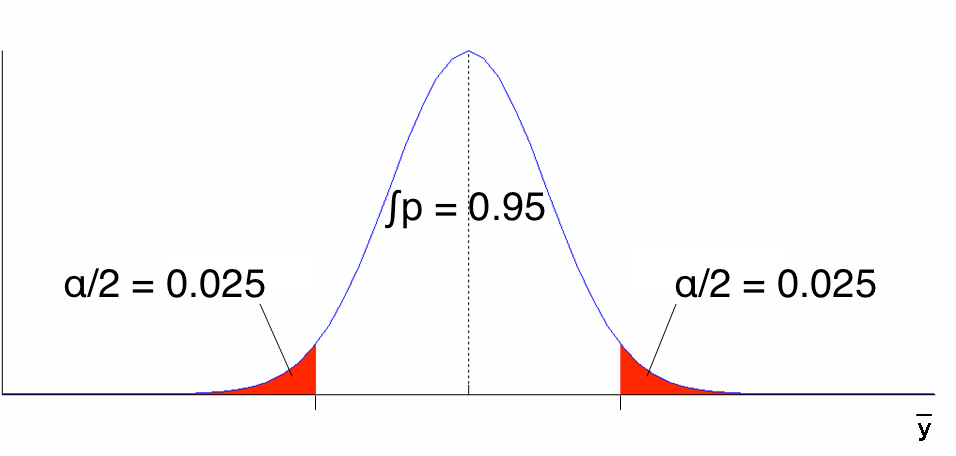
\includegraphics[width=0.5\textwidth]{../figs/alpha.png}};
\end{tikzpicture}
\end{ftst}

%=====

\begin{ftst}
{Inferential Errors}
{Type II error}
\begin{colorblock}{}{bg=green!30,fg=black}
\textbf{Type II error} (false negative): failure to reject the null hypothesis when it is false.
\end{colorblock}
\vone
The probability of occurrence of a false negative in any hypothesis testing procedure is generally represented by the Greek letter $\beta$:

\beqs 
\beta = P\left(\mbox{type II error}\right) = P\left(\mbox{not reject }H_0|H_0\mbox{ is false}\right)
\eqs

The quantity ($1-\beta$) is known as \textit{power} of the test, and quantifies its sensitivity to effects that violate the null hypothesis.
\end{ftst}

%=====

\begin{ftst}
{Inferential Errors}
{Type II error}
\begin{columns}[T]
	\column{0.55\textwidth}
		Unlike the Type-I error, the definition of the Type-II error rate requires further specification of the value of the parameter being investigated under the alternative hypothesis;
		\vone
		The probability of failing to reject a false $H_0$ is strongly dependent on the magnitude of the difference between the value under $H_0$ and the real value of the parameter.
	\column{0.45\textwidth}
	\end{columns}
\begin{tikzpicture}[remember picture,overlay]
\node[anchor=south east,yshift=130pt,xshift=-5pt] at (current page.south east) {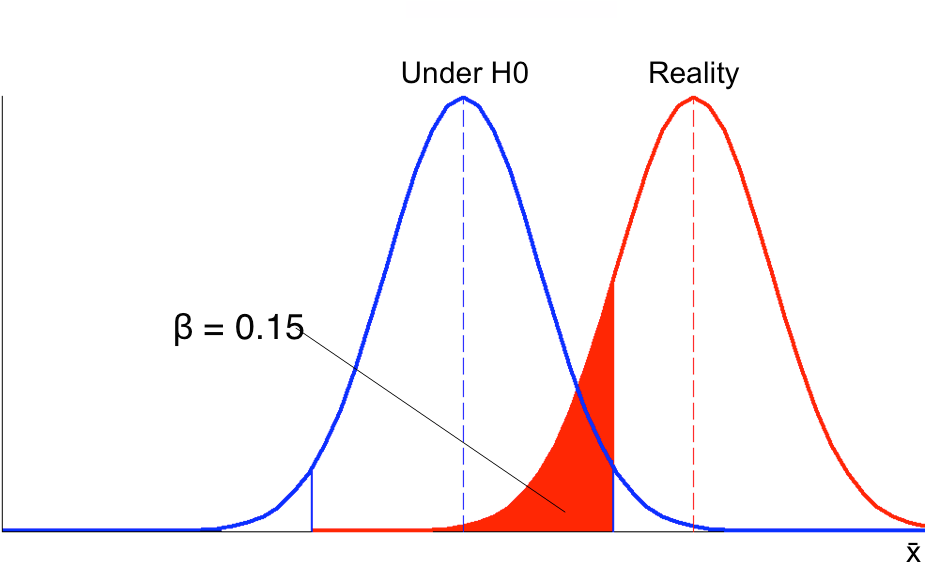
\includegraphics[width=0.45\textwidth]{../figs/beta-a.png}};
\node[anchor=south east,yshift=30pt,xshift=-5pt] at (current page.south east) {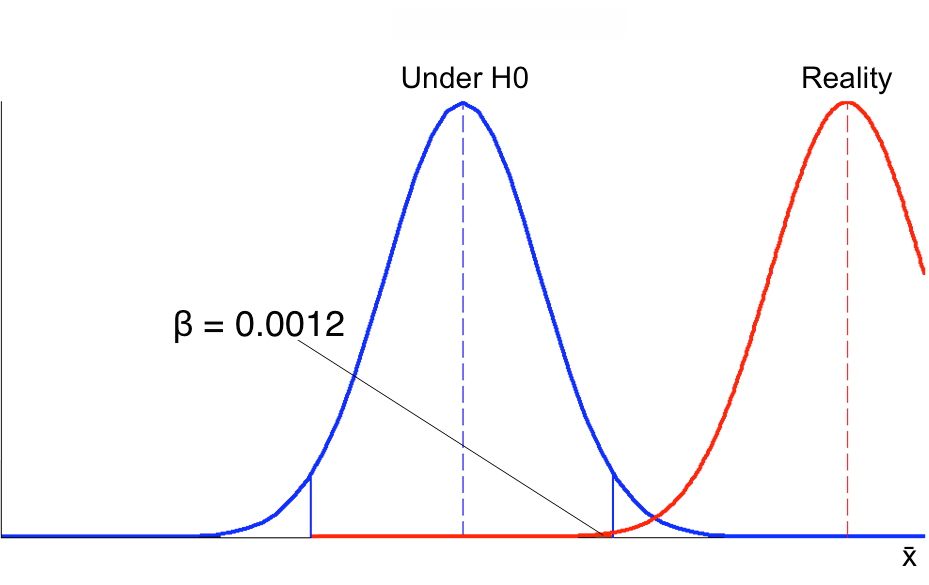
\includegraphics[width=0.45\textwidth]{../figs/beta-d.png}};
\end{tikzpicture}

\end{ftst}

%=====

\begin{ftst}
{Inferential Errors}
{Type II error}
The power of a test is governed by several factors:

\bitems Controllable: significance level, sample size, directionality of $H_1$;
	\item Uncontrollable: real value of the parameter, variance;
\eitem

If $H_0$ is false, the smaller the magnitude of the difference between the real value of the parameter and the one under the null hypothesis, the greater the probability of a type II error - \textbf{\textit{but the practical importance of the effect gets smaller}}.
\end{ftst}

%=====

\begin{ftst}
{Inferential Errors}
{Considerations}
\textbf{Type I error} ($\alpha$) depends only on the distribution of the null hypothesis - easier to control;
\vone
\textbf{Type II error} ($\beta$) depends on the real value of the parameter - more difficult to specify and control;
\vone
These characteristics lead to the following classification of the conclusions obtained from the test of hypotheses:
\begin{block}{}
\bitems Rejection of $H_0$ - \textit{strong} conclusion; 
\spitem Failure to reject $H_0$ - \textit{weak} conclusion (but we can fortify it);
\eitem
\end{block}
\vone
It is important to remember that failing to reject $H_0$ does not mean that there is evidence in favor of $H_0$ - it only suggests that it is a better model than the alternative.
\end{ftst}

%=====

\begin{ftst}
{Hypothesis Testing}
{General procedure}
\bitems Identify the parameter of interest;
	\item Define $H_0$ and $H_1$ (one- or two-sided);
	\item Determine desired $\alpha$, $\beta$;
	\item Define minimally interesting effect $\delta^*$;
	\item Calculate sample size;
	\item Determine the test statistic and critical region;
	\item Compute the statistic;
	\item Decide whether or not to reject $H_0$;
\eitem

\begin{tikzpicture}[remember picture,overlay]
\node[anchor=south east,yshift=2pt, xshift=-15pt] at (current page.south east) {\includegraphics[width=.21\textwidth]{../figs/hypothesis-wine.png}};
\end{tikzpicture}
\lfr{Image (c) Roots Run Deep Winery: \url{http://www.rootsrundeep.com/hypothesis.html}}
\end{ftst}

%=====

\begin{ftst}
{Hypothesis Testing}
{Mean of a normal distribution, variance known}
Back to the green peas example, we want to determine if there is any significant deviation on the mean weight of the sacks. Assume (for now) that the variance of the process is known. The test hypotheses are defined as:

\beqs\begin{cases}
H_0: \mu = 50kg\\
H_1: \mu \neq 50kg
\end{cases}\eqs
\vone
Let the desired significance level be $\alpha = 0.05$;
\vone
Given these characteristics, we expect that the sampling distribution of $\bar{X}$ is normal, with $Var(\bar{X})=\sigma^2/n$ and -- \textbf{if $H_0$ is true } -- a mean of $\mu_{\bar{X}}=\mu_0=50$;
\begin{tikzpicture}[remember picture,overlay]
\node[anchor=north east,yshift=12pt,xshift=-5pt] at (current page.north east) {
\includegraphics[width=0.2\textwidth]{../figs/peas.png}};
\end{tikzpicture}
\end{ftst}

%=====

\begin{ftst}
{Hypothesis Testing}
{Mean of a normal distribution, variance known}
Based on these characteristics, the standardized variable
\beqs Z_0 = \frac{\bar{X} - \mu_0}{\sigma/\sqrt{n}}\eqs
\vhalf
\noindent will be distributed according to the standard normal, $\mathcal{N}\left(0,1\right)$, \textbf{if $\mathbf{H_0}$ is true}.
\vhalf
This result implies that:
\beqs
P\left(z_{\alpha/2}\leq Z_0\leq z_{1-\alpha/2}\mid H_0~\mbox{is true}\right) = 1-\alpha
\eqs

\noindent which provides a selection criterion between $H_0$ and $H_1$:
\vhalf
\bitems If $z_{\alpha/2}> Z_0$ or $z_{1-\alpha/2}<Z_0$, reject $H_0$ with confidence $(1-\alpha)$;
	\spitem Otherwise, there is not enough evidence to reject $H_0$ at this confidence level;
\eitem
\begin{tikzpicture}[remember picture,overlay]
\node[anchor=north east,yshift=12pt,xshift=-5pt] at (current page.north east) {
\includegraphics[width=0.2\textwidth]{../figs/peas.png}};
\end{tikzpicture}
\end{ftst}

%=====

\begin{ftst}
{Hypothesis Testing}
{Mean of a normal distribution, variance known}
Assume that we got $\bar{x} = 49.65$kg from our $n=10$ observations, and that we know that $\sigma = 1$kg. In this case,

\beqs 
z_0 = \frac{49.65 - 50}{1/\sqrt{10}} = -1.113
\eqs
\vhalf
The critical values of the standard normal distribution at the significance level $\alpha = 0.05$ are $\left[z_{0.025},z_{0.975}\right] = \left[-1.96,1.96\right]$;
\vone
Since $z_0\in \left[-1.96,1.96\right]$, we can conclude that there is not enough evidence to reject $H_0$ at the $95\%$ confidence level.
\begin{tikzpicture}[remember picture,overlay]
\node[anchor=north east,yshift=12pt,xshift=-5pt] at (current page.north east) {
\includegraphics[width=0.2\textwidth]{../figs/peas.png}};
\end{tikzpicture}
\end{ftst}

%=====

\begin{ftst}
{Hypothesis Testing}
{Mean of a normal distribution, variance unknown}
Suppose now a more realistic situation in which the real variance is unknown. Besides, assume that we are interested in detecting only negative deviations from the nominal contents of the package.
\vone
The test hypotheses can be defined as:
\beqs\begin{cases}
H_0: \mu \geq 50kg\\
H_1: \mu < 50kg 
\end{cases}\eqs
\vhalf
Assume also that we want to be more conservative, so we pick a significance level $\alpha = 0.01$;
\vone
In this case, \textbf{if $H_0$ is true}, we have that
\beqs T_0 = \frac{\bar{X} - \mu_0}{S/\sqrt{n}} \sim t_{n-1}
\eqs
\begin{tikzpicture}[remember picture,overlay]
\node[anchor=north east,yshift=12pt,xshift=-5pt] at (current page.north east) {
\includegraphics[width=0.2\textwidth]{../figs/peas.png}};
\end{tikzpicture}
\end{ftst}

%=====

\begin{ftst}
{Hypothesis Testing}
{Mean of a normal distribution, variance unknown}
From the same data used earlier, $\bar{x} = 49.65$kg, $n=10$, $s = 0.697$kg:
\beqs t_0 = \frac{49.65 - 50}{0.697/\sqrt{10}} = -1.597\eqs
\vhalf
The critical value of this test statistic for the desired significance is $t_{\alpha,n-1} = t_{0.01,9} = -2.82$, which means that under $H_0$ there is a $99\%$ change that the test statistic will yield a value greater than this number.
\vone
Given that $t_0 > -2.82$, we conclude that the evidence is insufficient to reject $H_0$ at the $99\%$ confidence level;
\begin{tikzpicture}[remember picture,overlay]
\node[anchor=north east,yshift=12pt,xshift=-5pt] at (current page.north east) {
\includegraphics[width=0.2\textwidth]{../figs/peas.png}};
\end{tikzpicture}
\end{ftst}

%=====

\begin{ftstf}
	{Hypothesis Testing}
	{Mean of a normal distribution, variance unknown}
	\begin{rcode}
> sample <- as.numeric(scan("../data files/greenpeas.txt"))

> t.test(sample,
+        alternative = "less",
+        mu = 50,
+        conf.level = 0.99)

One Sample t-test
data:  sample
t = -1.5969, df = 9, p-value =0.07237
alternative hypothesis: true mean is less than 50
99 percent confidence interval:
-Inf 50.2699
sample estimates:
mean of x 
49.648
	\end{rcode}
	\begin{tikzpicture}[remember picture,overlay]
	\node[anchor=north east,yshift=-70pt,xshift=-5pt] at (current page.north east) {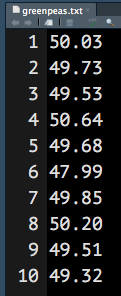
\includegraphics[width=0.22\textwidth]{../figs/peastxt.png}};
	\node[anchor=north east,yshift=12pt,xshift=-5pt] at (current page.north east) {
\includegraphics[width=0.2\textwidth]{../figs/peas.png}};
	\end{tikzpicture}
\end{ftstf}

%=====

\begin{ftst}
{Hypothesis Testing}
{Reporting results}
Description of the results:
\vone
\begin{block}{}
\centering\textit{(In)Sufficient evidence for rejecting $H_0$\\at the significance level $\alpha$.}
\end{block}
\vone
Even thought it is correct, this description is relatively poor:

\bitems It does not provide information on the intensity of the evidence for rejection/non-rejection;
	\item It imposes a predetermined significance level to the consumer of the information;
	\item Does not provide information the magnitude of the effect found or the sensitivity of the test.
\eitem
\end{ftst}

%=====

\begin{ftst}
{Hypothesis Testing}
{The p-value}
\begin{colorblock}{}{bg=green!30,fg=black}
\centering\textbf{p-value}: \textit{the lowest significance level that would lead\\to the rejection of $H_0$for the available data.}
\end{colorblock}
\vone
Can be interpreted as the probability under $H_0$ of the test statistic assuming a value at least as extreme as the one obtained;
\vone\vhalf
For the previous example, the p-value could be calculated as:
\beqs
p = P(t_0\leq -1.597|H_0 = \mbf{TRUE}) = \int\limits_{-\infty}^{-1.597}t_{(df=9)}dt = 0.07237
\eqs
\vhalf

\begin{block}{}
\centering\textit{A priori} definition of the significance level is still important!
\end{block}
\end{ftst}

%=====

\begin{ftst}
{Hypothesis Testing}
{p-values, significance and effect sizes}
Statistical $\times$ practical significance: p-values can be made arbitrarily small, if $n$ is big enough;
\vone 
As an example, suppose a test of $H_0: \mu=500$ against a two-sided alternative, with $n=5000, \bar{x}=499,\ s=5$. In this case we would have:

\bitems $t_0 = -14.142$;
\item $p = 1.02\times 10^{-23}$;\eitem
\vone	
Is it really \textit{that} significant?
\end{ftst}

%=====

\begin{ftst}
{Hypothesis Testing}
{p-values, significance and effect sizes}
To ``tell the whole story'' of the experiment, it is necessary to use \textbf{effect size estimators} alongside the tests of statistical significance; 
\vone
While there are whole books on the subject\footnote[3]{\tiny See, for instance, Paul D. Ellis' \textit{The Essential Guide to Effect Sizes}, Cambridge University Press, 2010.}, the main idea is quite simple - to quantify the magnitude of the observed deviation from the null hypothesis.
\vone
Examples of effect size estimators include the simple point estimator for the difference $\bar{x} - \mu_0$, or the dimensionless \textit{d} estimator:

\beqs
d = \frac{\bar{x}-\mu_0}{s}
\eqs

\noindent which quantifies the difference in terms of sample standard deviations.
\vone
\end{ftst}

%=====

\begin{ftstf}
{Hypothesis Testing}
{p-values, effects sizes and confidence intervals}
\begin{block}{}
\centering\textit{Point estimators + confidence intervals quantify the magnitude and accuracy of effects, and must be reported alongside the results of significance testing whenever possible.}
\end{block}
\vhalf
Suppose we are testing $H_0: \mu=50$ against the two-sided alternative hypothesis, with $n=10$ and $\alpha=0.01$. Assume that the population is known to be normal, with unknown variance. We'll use the same data as before:
\vhalf
\begin{rcode}
> t.test(sample, mu = 50, conf.level = 0.99)
(...)
t = -1.5969, df = 9, p-value = 0.1447
alternative hypothesis: true mean is not equal to 50
99 percent confidence interval:
 48.93166 50.36434
sample estimates:
mean of x 
   49.648 
\end{rcode}
\begin{tikzpicture}[remember picture,overlay]
\node[anchor=north east,yshift=12pt,xshift=-5pt] at (current page.north east) {
\includegraphics[width=0.2\textwidth]{../figs/peas.png}};
\end{tikzpicture}
\end{ftstf}

%=====

\begin{ftst}{Sample size and Type-II error}
{Some considerations}
The probability of Type-II error can be easily (and often wrongly) evaluated \textit{a posteriori}, but its definition \textit{a priori} requires some care;
\vone
Given a desired test, its power is essentially a function of 4 elements:
\bitems Actual size of the difference;
	\item Variability of the observations;
	\item Significance level;
	\item Sample size.
\eitem
\vone
The experimenter generally have very little control over the first two.
\end{ftst}

%=====

\begin{ftst}{Sample size and Type-II error}
{Some considerations}
A strategy for estimating an effective lower bound for the power of a test includes a definition of an \textit{minimally interesting effect} $\delta^*$. 
\vone
This value must be derived from technical and scientific knowledge about the phenomenon or system under experimentation. 
\vhalf
\begin{block}{}
\centering It is essential to have a good understanding of the field in which the experiment will be conducted.
\end{block}
\vhalf
Once $\delta^*$ is defined, the experimenter can obtain an estimate of the variability of observations (e.g., by a pilot study), which can then be used to obtain an approximate power value for the experiment;
\end{ftst}

%=====

\begin{ftst}
{Sample size and Type-II error}
{Some considerations}
Having obtained this estimation of the Type-II error probability, one can run his/her experiment with a better understanding of its ability to detect effects of interest.
\vone
The test will have lower power for differences smaller than $\delta^*$, but these differences are below the minimally interesting effect; any effect greater than $\delta^*$ will result in a higher power for the test;
\vone
This technique can also be used as a way to compute the maximum necessary sample size for the experiment.
\end{ftst}

%=====

\begin{ftstf}
{Sample size and Type-II error}
{Example}
Suppose that on the green peas example we are really interested in detecting negative deviations from the nominal value greater than $1\%$, i.e., $\delta^* = 0.01\times 50 = 0.5$kg. The researcher defines that, for this minimally interesting effect, a test power of $0.85$ is desired. The desired significance is $\alpha = 0.01$.
\vone
The same sample of $n=10$ sacks is used. Assume that you estimated a reasonable standard deviation for this sample as $s=1$kg. From this data, we can compute the power of this test as:
\begin{columns}
\column[T]{0.5\textwidth}
\begin{rcode}
> s <- sd(sample)
> power.t.test(n = 10, 
+        delta = 0.5, 
+        sd = 1, 
+        sig.level = 0.01, 
+        type = "one.sample", 
+        alternative = "one.sided")
\end{rcode}
\column[T]{0.5\textwidth}
\begin{rcode}
One-sample t test power calculation 
n = 10
delta = 0.5
sd = 1
sig.level = 0.01
power = 0.1654013
alternative = one.sided
\end{rcode}
\end{columns}
\begin{tikzpicture}[remember picture,overlay]
\node[anchor=north east,yshift=12pt,xshift=-5pt] at (current page.north east) {
\includegraphics[width=0.2\textwidth]{../figs/peas.png}};
\node[anchor=south east,yshift=31pt,xshift=-75pt] at (current page.south east) {\footnotesize\color{red}$\boldsymbol{\longleftarrow}$};
\end{tikzpicture}
\end{ftstf}

%=====

\begin{ftstf}
{Sample size and Type-II error}
{Example}
What is the smallest sample size needed to obtain the desired power of $0.85$?
\vhalf
\begin{rcode}
> power.t.test(power = 0.85, delta = 0.5, sd = 1, sig.level = 0.01,
               type = "one.sample", alternative = "one.sided")

One-sample t test power calculation 
n = 47.98044
delta = 0.5
sd = 1
sig.level = 0.01
power = 0.85
alternative = one.sided
\end{rcode}
\vhalf
We need at least 48 observations to detect a $-5g\ (1\%)$ or larger deviation on the mean weight of the green peas packages with a power level of $0.85$.
\begin{tikzpicture}[remember picture,overlay]
\node[anchor=north east,yshift=12pt,xshift=-5pt] at (current page.north east) {
\includegraphics[width=0.2\textwidth]{../figs/peas.png}};
\node[anchor=south east,yshift=140pt,xshift=-182pt] at (current page.south east) {\footnotesize\color{red}$\mbf{\longleftarrow}$ \textbf{(round this value up)}};
\end{tikzpicture}
\end{ftstf}

\begin{ftst}
{Model validation}
{The normality assumption}
The assumption of normality, required for the \textbf{z} and \textbf{t} tests, needs to be validated.
	\begin{colorblock}{}{bg=green!30,fg=black}
	``\textit{The Assumption of Normality (note the upper case) that underlies parametric stats does not assert that the observations within a given sample are normally distributed, nor does it assert that the values within the population (from which the sample was taken) are normal. This core element of the Assumption of Normality asserts that \textbf{the distribution of sample means (across independent samples) is normal.}}''\\
	\flushright -- J. Toby Mordkoff, 2011.$^{(a)}$
	\end{colorblock}

\lfr{$^{(a)}$ Check J.T. Mordkoff's \textit{The assumption(s) of normality} for a nice discussion on this topic: \url{http://goo.gl/Z3w8ku}}
\end{ftst}

%=====

\begin{ftstf}
{Model validation}
{The normality assumption}
If the conditions for the CLT cannot be assumed \textit{a priori}, then normality tests can be performed on the data.
\vone
Graphical/qualitative tests;
\vone
\begin{rcode}
> library(car)
> qqPlot(sample,
+        pch=16,
+        cex=1.5,
+        las=1)
\end{rcode}
\begin{tikzpicture}[remember picture,overlay]
\node[anchor=south east,yshift=-10pt,xshift=10pt] at (current page.south east) {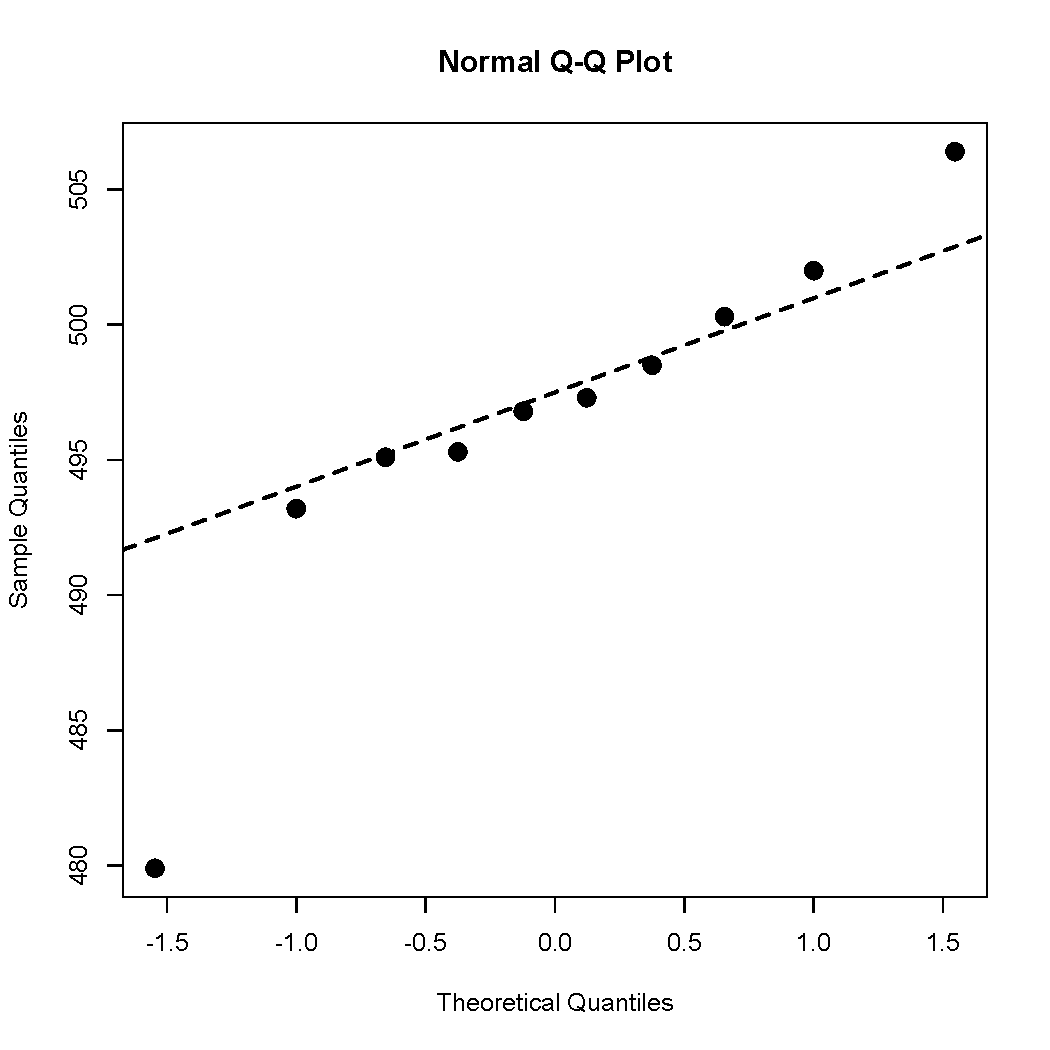
\includegraphics[width=.7\textwidth]{../figs/GraphNorm.pdf}};
\node[anchor=south east,yshift=42pt,xshift=-120pt] at (current page.south east) {\color{red}$\boldsymbol{\longleftarrow}$ \textit{outlier}?};
\node[anchor=north east,yshift=12pt,xshift=-5pt] at (current page.north east) {
\includegraphics[width=0.2\textwidth]{../figs/peas.png}};
\end{tikzpicture}
\end{ftstf}

%=====

\begin{ftst}
{Model validation}
{The normality assumption}
Analytical tests of normality (choose \textbf{one});
\bitems Shapiro-Wilk;
	\item Anderson-Darling;
	\item Lilliefors / Kolmogorov-Smirnov;
\eitem
\vone
These procedures use different aspects of the sample distribution to test the following hypotheses:
\beqs\begin{cases}
	H_0: \mbox{population is normal}\\
	H_1: \mbox{population is not normal}
\end{cases}\eqs
\vhalf
In this case, rejection of the null hypothesis suggests evidence that the \textbf{sample} came from a non-normal population. Generally we use a strict $\alpha$ threshold for these tests, and consider their results together with a graphical analysis.
\end{ftst}

%=====

\begin{ftstf}
{Model validation}
{The normality assumption}
Even thought the Lilliefors / Kolmogorov-Smirnov test is possibly the most widely used for normality testing, the Shapiro-Wilk test is recommended as a better alternative in Michael Crawley's \textit{The R Book}, and will be used throughout this course.
\vhalf
\begin{rcode}
> shapiro.test(sample)

Shapiro-Wilk normality test
data:  sample
W = 0.8809, p-value = 0.1335
\end{rcode}
\begin{tikzpicture}[remember picture,overlay]
\node[anchor=north east,yshift=12pt,xshift=-5pt] at (current page.north east) {
\includegraphics[width=0.2\textwidth]{../figs/peas.png}};
\end{tikzpicture}
\end{ftstf}

%=====

\begin{ftstf}
{Model validation}
{The independence assumption}
Possibly the strongest assumption of the statistical model used for the t-test is that of independence, that is, of the absence of unmodeled biases contaminating the data.
\vhalf
While I know of no procedure to test independence in the general case, the special case of serial autocorrelations in the data (which can emerge, for instance, as a consequence of heating effects or equipment degradation) can be tested by a procedure known as the Durbin-Watson test:
\begin{rcode}
> library(car)
> durbinWatsonTest(lm(sample ~ 1))

lag Autocorrelation D-W Statistic p-value
1      -0.0848535      2.111733   0.898
Alternative hypothesis: rho != 0
\end{rcode}
\begin{tikzpicture}[remember picture,overlay]
\node[anchor=north east,yshift=12pt,xshift=-5pt] at (current page.north east) {
\includegraphics[width=0.2\textwidth]{../figs/peas.png}};
\end{tikzpicture}
\end{ftstf}

%=====

\begin{ftstf}
{Model validation}
{The independence assumption}
The Durbin-Watson test depends on the ordering of the data, so observations should be ordered (either in the data file or by manipulating the data vector) according to covariates that are suspected to introduce dependencies, e.g., order of collection, placement criteria, etc.
\vone
Violations of the independence assumption tend to be the hardest to weed out, so extra care is recommended in the design of the experiment in order to prevent, control, or at least document all variables that could introduce dependencies in the data.
\end{ftstf}

%=====

\begin{ftst}
{The green peas experiment}
{Going over the process}
After examining the green peas example, it is interesting to go back and follow the recommended sequence for this kind of experiment:

\bitems Formulate question of interest;
	\spitem Define minimally interesting effect;
	\spitem Define desired confidence and power;
	\spitem Calculate required sample size;
	\spitem Collect data;
	\spitem Perform statistical analysis;
	\spitem Draw conclusions and recommendations.
\eitem
\begin{tikzpicture}[remember picture,overlay]
\node[anchor=north east,yshift=12pt,xshift=-5pt] at (current page.north east) {
\includegraphics[width=0.2\textwidth]{../figs/peas.png}};
\end{tikzpicture}
\end{ftst}

%=====


\begin{ftst}
{Bibliography}
{\ }
\scriptsize
\textbf{Required reading}

\benums D.C. Montgomery, G.C. Runger, \textit{Applied Statistics and Probability for Engineers}, Ch. 9.\\5th ed., Wiley, 2010. 
\item J.T. Mordkoff (2011), \textit{The assumption(s) of normality} - \url{http://goo.gl/Z3w8ku}
\eenum

\textbf{Recommended reading}

\benums A. Reinhart, \textit{Statistics Done Wrong: the woefully complete guide} - {\tiny\url{http://www.statisticsdonewrong.com}}
\item W. Thalheimer and S. Cook, \textit{How to calculate effect sizes from published research articles: A simplified methodology} - {\tiny\url{http://goo.gl/c0g1oK}}
\item E. Ernst and S. Singh, \textit{Trick or Treatment}, Norton \& Company, 2009.
\eenum
\end{ftst}

%=====

\begin{ftstf}{About this material}{Conditions of use and referencing}
\centering\footnotesize This work is licensed under the Creative Commons CC BY-NC-SA 4.0 license\\(Attribution Non-Commercial Share Alike International License version 4.0).\\
\vhalf
\url{http://creativecommons.org/licenses/by-nc-sa/4.0/}\\
\vone
\footnotesize Please reference this work as:\\
\footnotesize \flushleft Felipe Campelo (2018), \textit{Lecture Notes on Design and Analysis of Experiments}.\\Online: {\scriptsize\url{https://github.com/fcampelo/Design-and-Analysis-of-Experiments}}\\
Version 2.12. Creative Commons BY-NC-SA 4.0.\\

\begin{Verbatim}[fontsize=\tiny]
    @Misc{Campelo2018,
      title={Lecture Notes on Design and Analysis of Experiments},
      author={Felipe Campelo},
      howPublished={\url{https://github.com/fcampelo/Design-and-Analysis-of-Experiments}},
      year={2018},
      note={Version 2.12. Creative Commons BY-NC-SA 4.0.},
    }
\end{Verbatim}

\begin{tikzpicture} [remember picture,overlay]
\node[anchor=south,yshift=0pt] at (current page.south){ \includegraphics[width=.2\textwidth]{../figs/CCSomerights.png}};
\end{tikzpicture}
\end{ftstf}



\end{document}